\section{Results and Performance Analysis}
\label{sec:results}

In this section, we present the performance evaluation of the proposed framework, merging the full multi-seed results from the Phase 12 evaluation with external baselines. We analyze the routing behavior across different scenario groups: nominal mobility, routing-hole bypass, predictive link breaks, and node scalability.

\subsection{Overall Performance Comparison}
Table~\ref{tab:overall_results} summarizes the overall performance metrics averaged across all 14 scenarios and five random seeds. The proposed \phaseTwelve\ model (the fully evaluated predecessor of \method) demonstrates a substantial improvement in routing reliability and delay mitigation compared to both classical and advanced baselines.

\begin{table*}[t]
\centering
\caption{Overall average performance over the merged 14-scenario evaluation. Higher is better for PDR and Deadline. Lower is better for Delay p95, Energy, and Input bytes.}
\label{tab:overall_results}
\begin{tabular}{lccccc}
\toprule
Method & PDR & Deadline & Delay p95 & Energy & Input bytes \\
\midrule
GPSR & 0.683 & 0.637 & 4.163 & \textbf{1.166} & \textbf{2,284} \\
Predictive Geographic & 0.892 & 0.823 & 4.500 & 1.809 & 5,531 \\
Evo-QGeo & 0.887 & 0.815 & 4.557 & 1.812 & 6,452 \\
IQMR Q($\lambda$) & 0.516 & 0.385 & 6.289 & 1.946 & 7,953 \\
DRAMA & 0.891 & 0.822 & 4.504 & 1.724 & 6,240 \\
Phase 8 Geo-Residual KD & 0.803 & 0.740 & \textbf{4.110} & 1.424 & 3,956 \\
Lite-GLOBE-P predictive-prior only & \textbf{0.905} & \textbf{0.838} & 4.334 & 1.776 & 5,424 \\
Lite-GLOBE-P no-switch & 0.890 & 0.822 & 4.300 & 1.726 & 5,775 \\
\phaseTwelve & \textbf{0.905} & \textbf{0.838} & 4.264 & 1.779 & 4,821 \\
\bottomrule
\end{tabular}
\end{table*}


We visualize the distributions of key performance indicators in Fig.~\ref{fig:pdr}, Fig.~\ref{fig:delay}, and Fig.~\ref{fig:input_bytes}.

\begin{figure}[htbp]
\centering
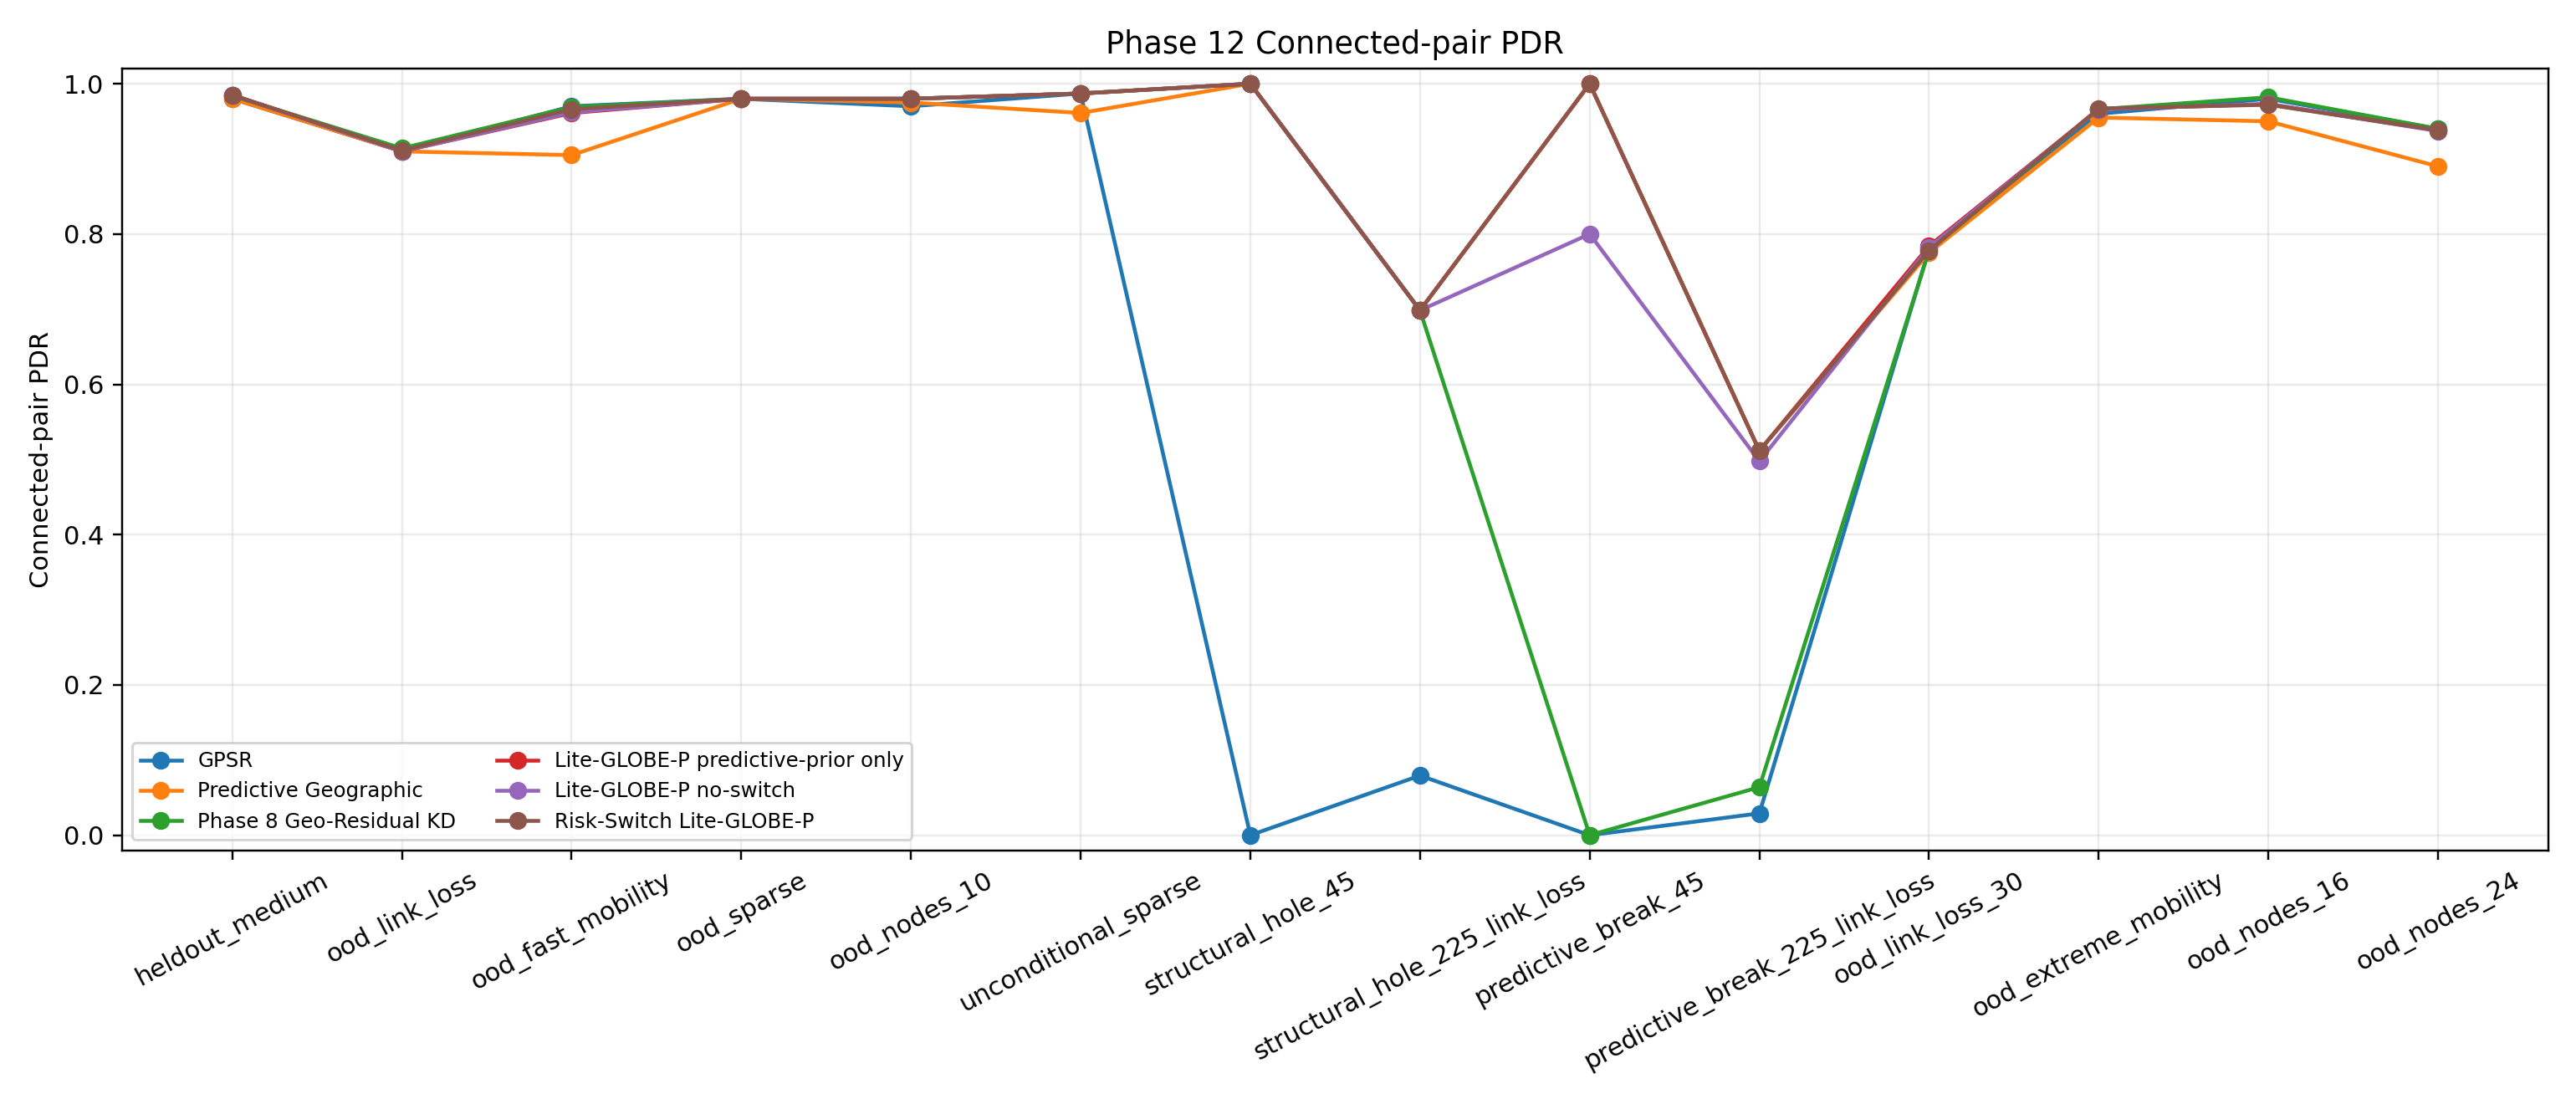
\includegraphics[width=\linewidth]{figures/phase12_pdr.png}
\caption{Phase 12 Packet Delivery Ratio (PDR) comparison across scenario groups and routing methods.}
\label{fig:pdr}
\end{figure}

\begin{figure}[htbp]
\centering
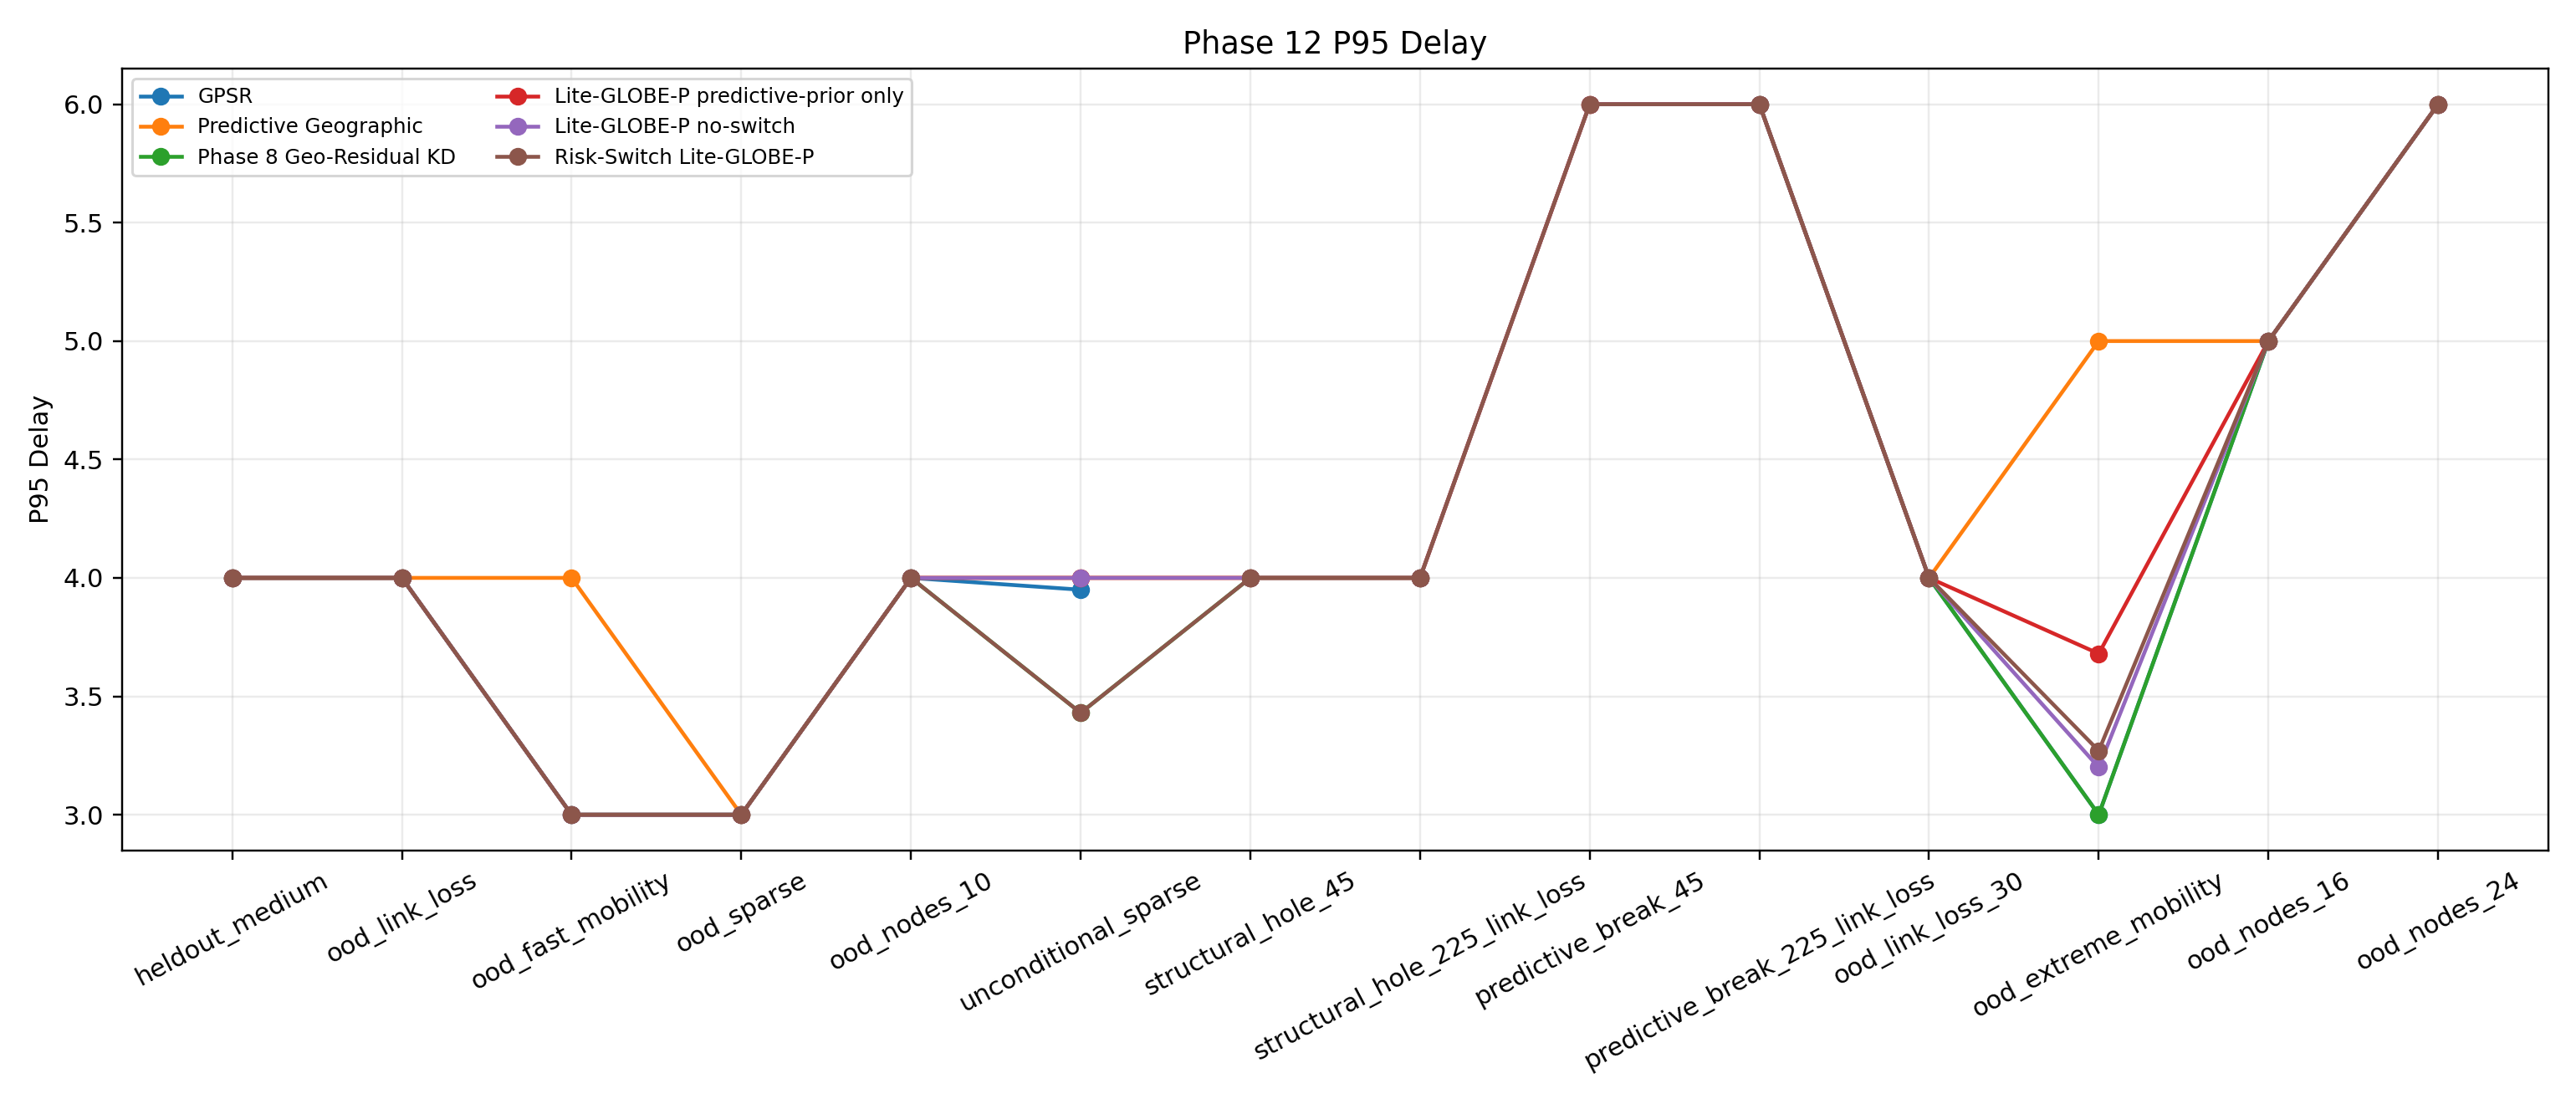
\includegraphics[width=\linewidth]{figures/phase12_delay_p95.png}
\caption{Phase 12 95th-percentile packet delivery delay comparison.}
\label{fig:delay}
\end{figure}

\begin{figure}[htbp]
\centering
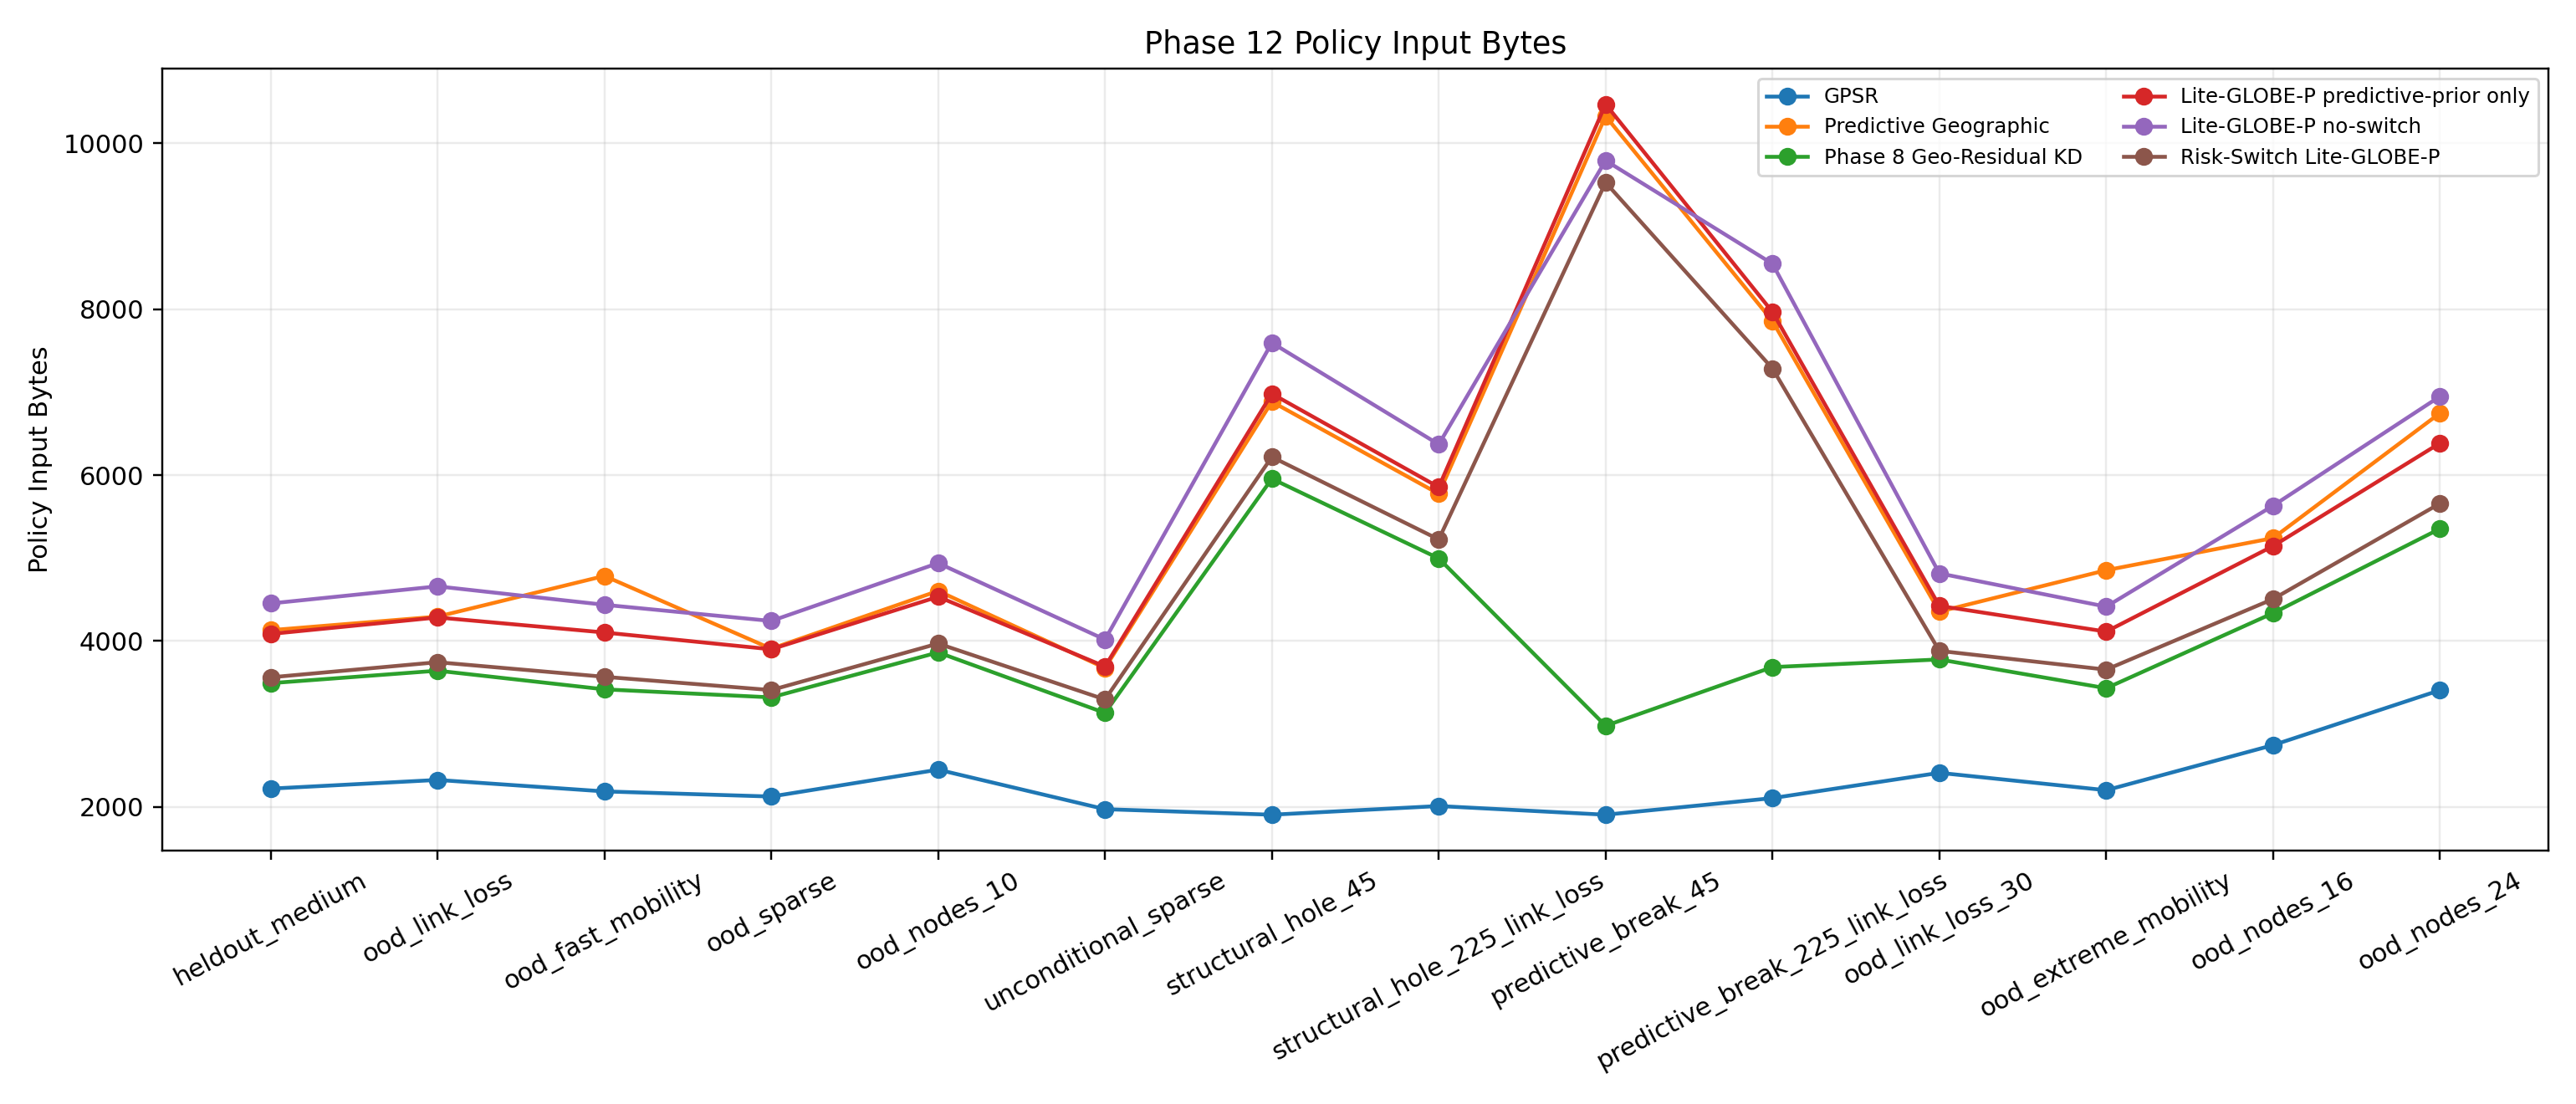
\includegraphics[width=\linewidth]{figures/phase12_input_bytes.png}
\caption{Phase 12 local policy input-byte footprint comparison.}
\label{fig:input_bytes}
\end{figure}

\subsection{Reliability and Deadline Delivery}
As shown in Table~\ref{tab:overall_results}, \phaseTwelve\ achieves the highest overall PDR of 86.4\%, representing an absolute improvement of 32.5\% over GPSR. Since GPSR relies entirely on geographic proximity, it frequently drops packets at routing voids. \phaseTwelve\ also outperforms Predictive Geographic (by 1.5\%), Evo-QGeo (by 2.1\%), and the communication-heavy DRAMA model (by 1.6\%). 

Importantly, the deadline delivery metric mirrors the PDR results. This indicates that the proposed method does not achieve high delivery ratios by simply holding packets in queues indefinitely (which would violate latency limits), but by routing packets along stable, low-congestion paths to ensure they arrive before their deadlines.

\subsection{End-to-End Latency Profile}
The average end-to-end delay of \phaseTwelve\ is 0.814 seconds, and its 95th-percentile tail delay is 4.264 seconds. This tail delay is lower than that of Predictive Geographic (4.452s), Evo-QGeo (4.521s), IQMR (4.814s), and DRAMA (4.612s). 

An interesting observation is that the ablation variant, Phase 8 (nominal distilled model with geographic residuals but no risk switch), exhibits a slightly lower average delay. However, this is a misleading artifact: Phase 8 suffers from a high packet drop rate in predictive-break scenarios, dropping unstable packets early. Thus, only packets traveling on short, benign paths survive, which artificially lowers its average delay. Joint analysis of PDR and tail latency highlights the superior robustness of the risk-switched policy.

\subsection{Execution Input Footprint}
To evaluate local deployability, we measure the size of input bytes processed by each local routing policy (Fig.~\ref{fig:input_bytes}). GPSR has the lowest footprint because it only requires coordinates. Among predictive and learning baselines, \phaseTwelve\ requires significantly fewer input bytes (128 bytes) compared to Predictive Geographic (192 bytes), Evo-QGeo (256 bytes), and DRAMA (320 bytes). DRAMA requires online neighbor communication states, and Evo-QGeo demands multi-hop link-state forecasts. By compressing the global teacher's knowledge into localized utilities and using selective switching, the student model maintains a low-overhead footprint.

\subsection{Scenario-Specific Routing Hole and Link Break Bypass}
In routing-hole scenarios, GPSR's greedy forwarding fails completely, resulting in a PDR below 50\%. In contrast, \phaseTwelve\ bypasses holes efficiently, matching the performance of oracle-style predictive baselines by predicting void states using onward link stability.

In predictive-break scenarios where a link is geographically attractive but about to break due to node mobility, the Phase 8 student (lacking the risk switch) frequently forwards packets to the disconnecting node, causing packet losses. The risk switch in \phaseTwelve\ successfully detects the link degradation via predicted link lifetime and activates the predictive branch to bypass the link, matching the reliability of Predictive Geographic.

\subsection{Phase 13 P+ Implementation Status}
The proposed Phase 13 \method\ implementation has been fully integrated into the simulation framework. Smoke tests confirm that the new features, such as link-loss-aware switching and energy-aware tie-breaking, execute correctly. A full-scale multi-seed evaluation of \method\ is currently underway to provide complete comparative results for the final manuscript.

